%!TEX root = coatli.tex

\chapter{Telescope}
\label{chapter:telescope}

\section{Optics}

\begin{table}
\begin{center}
\caption{Telescope Optical Parameters}
\label{table:telescope-optical-parameters}
\medskip
\footnotesize
\begin{tabular}{llccc}
\hline
\hline
Component&Parameter&Value\\
\hline
M1
&Clear Aperture Diameter (mm)     &500\\
&Radius of Curvature (mm)         &$-2554.7$\\
&Focal Length (mm)&$-1277$\\
&Focal Ratio                      &$f/2.555$\\
&Conic Constant                   &$-1.05$\\
&Central Hole Diameter (mm)       &120\\
\hline
M2
&Clear Aperture Diameter (mm)     &160\\
&Radius of Curvature (mm)         &$-1137.2$\\
&Focal length (mm) &$-569$\\
&Focal Ratio                      &$f/3.554$\\
&Conic Constant                   &$-4.346$\\
&Baffle Diameter (mm)             &180\\
\hline
M1+M2 
&Focal Length (mm)&$-3967$\\
&Focal Ratio&$f/7.933$\\
&Vertex of M1 to Vertex of M2 (mm)&$-891.85$\\
&Vertex of M1 to Focal Plane (mm) &300\\
&Flange to Focal Plane (mm)       &136\\
\hline
\end{tabular}
\end{center}
\end{table}

The COATLI telescope is a 50-cm $f/8$ Ritchey-Crétien supplied by ASTELCO. 

The optics originally supplied in 2016 performed poorly and never gave images better than about 1.4 arcsec FWHM. We received new optics in 2020, tested them extensively in CU, and installed them in November 2021. The adopted parameters of the 2020 optics are given in Table~\ref{table:telescope-optical-parameters}. 

The mirrors are fabricated in an unspecified low-expansion glass and coated with aluminium protected with a layer of MgF$_2$.

\section{Mechanics}

The primary mirror cell is mainly carbon fiber, with an aluminum dovetail and instrument flange. The telescope nominal focal plane is 136 mm below the instrument flange.

Carbon fiber Serrutier struts support the aluminum secondary ring. The structs have ball-and-socket joints at both ends, which help maintain collimation at different pointings. 

The telescope is equipped with a motorized focuser for the secondary. 

The primary mirror can be adjusted in tilt, the secondary mirror in center and tilt, and the primary baffle in tilt with respect to the primary. 

Figures~\ref{figure:telescope-plans-first} to \ref{figure:telescope-plans-last} show plans of the telescope.

\begin{figure}
\begin{center}
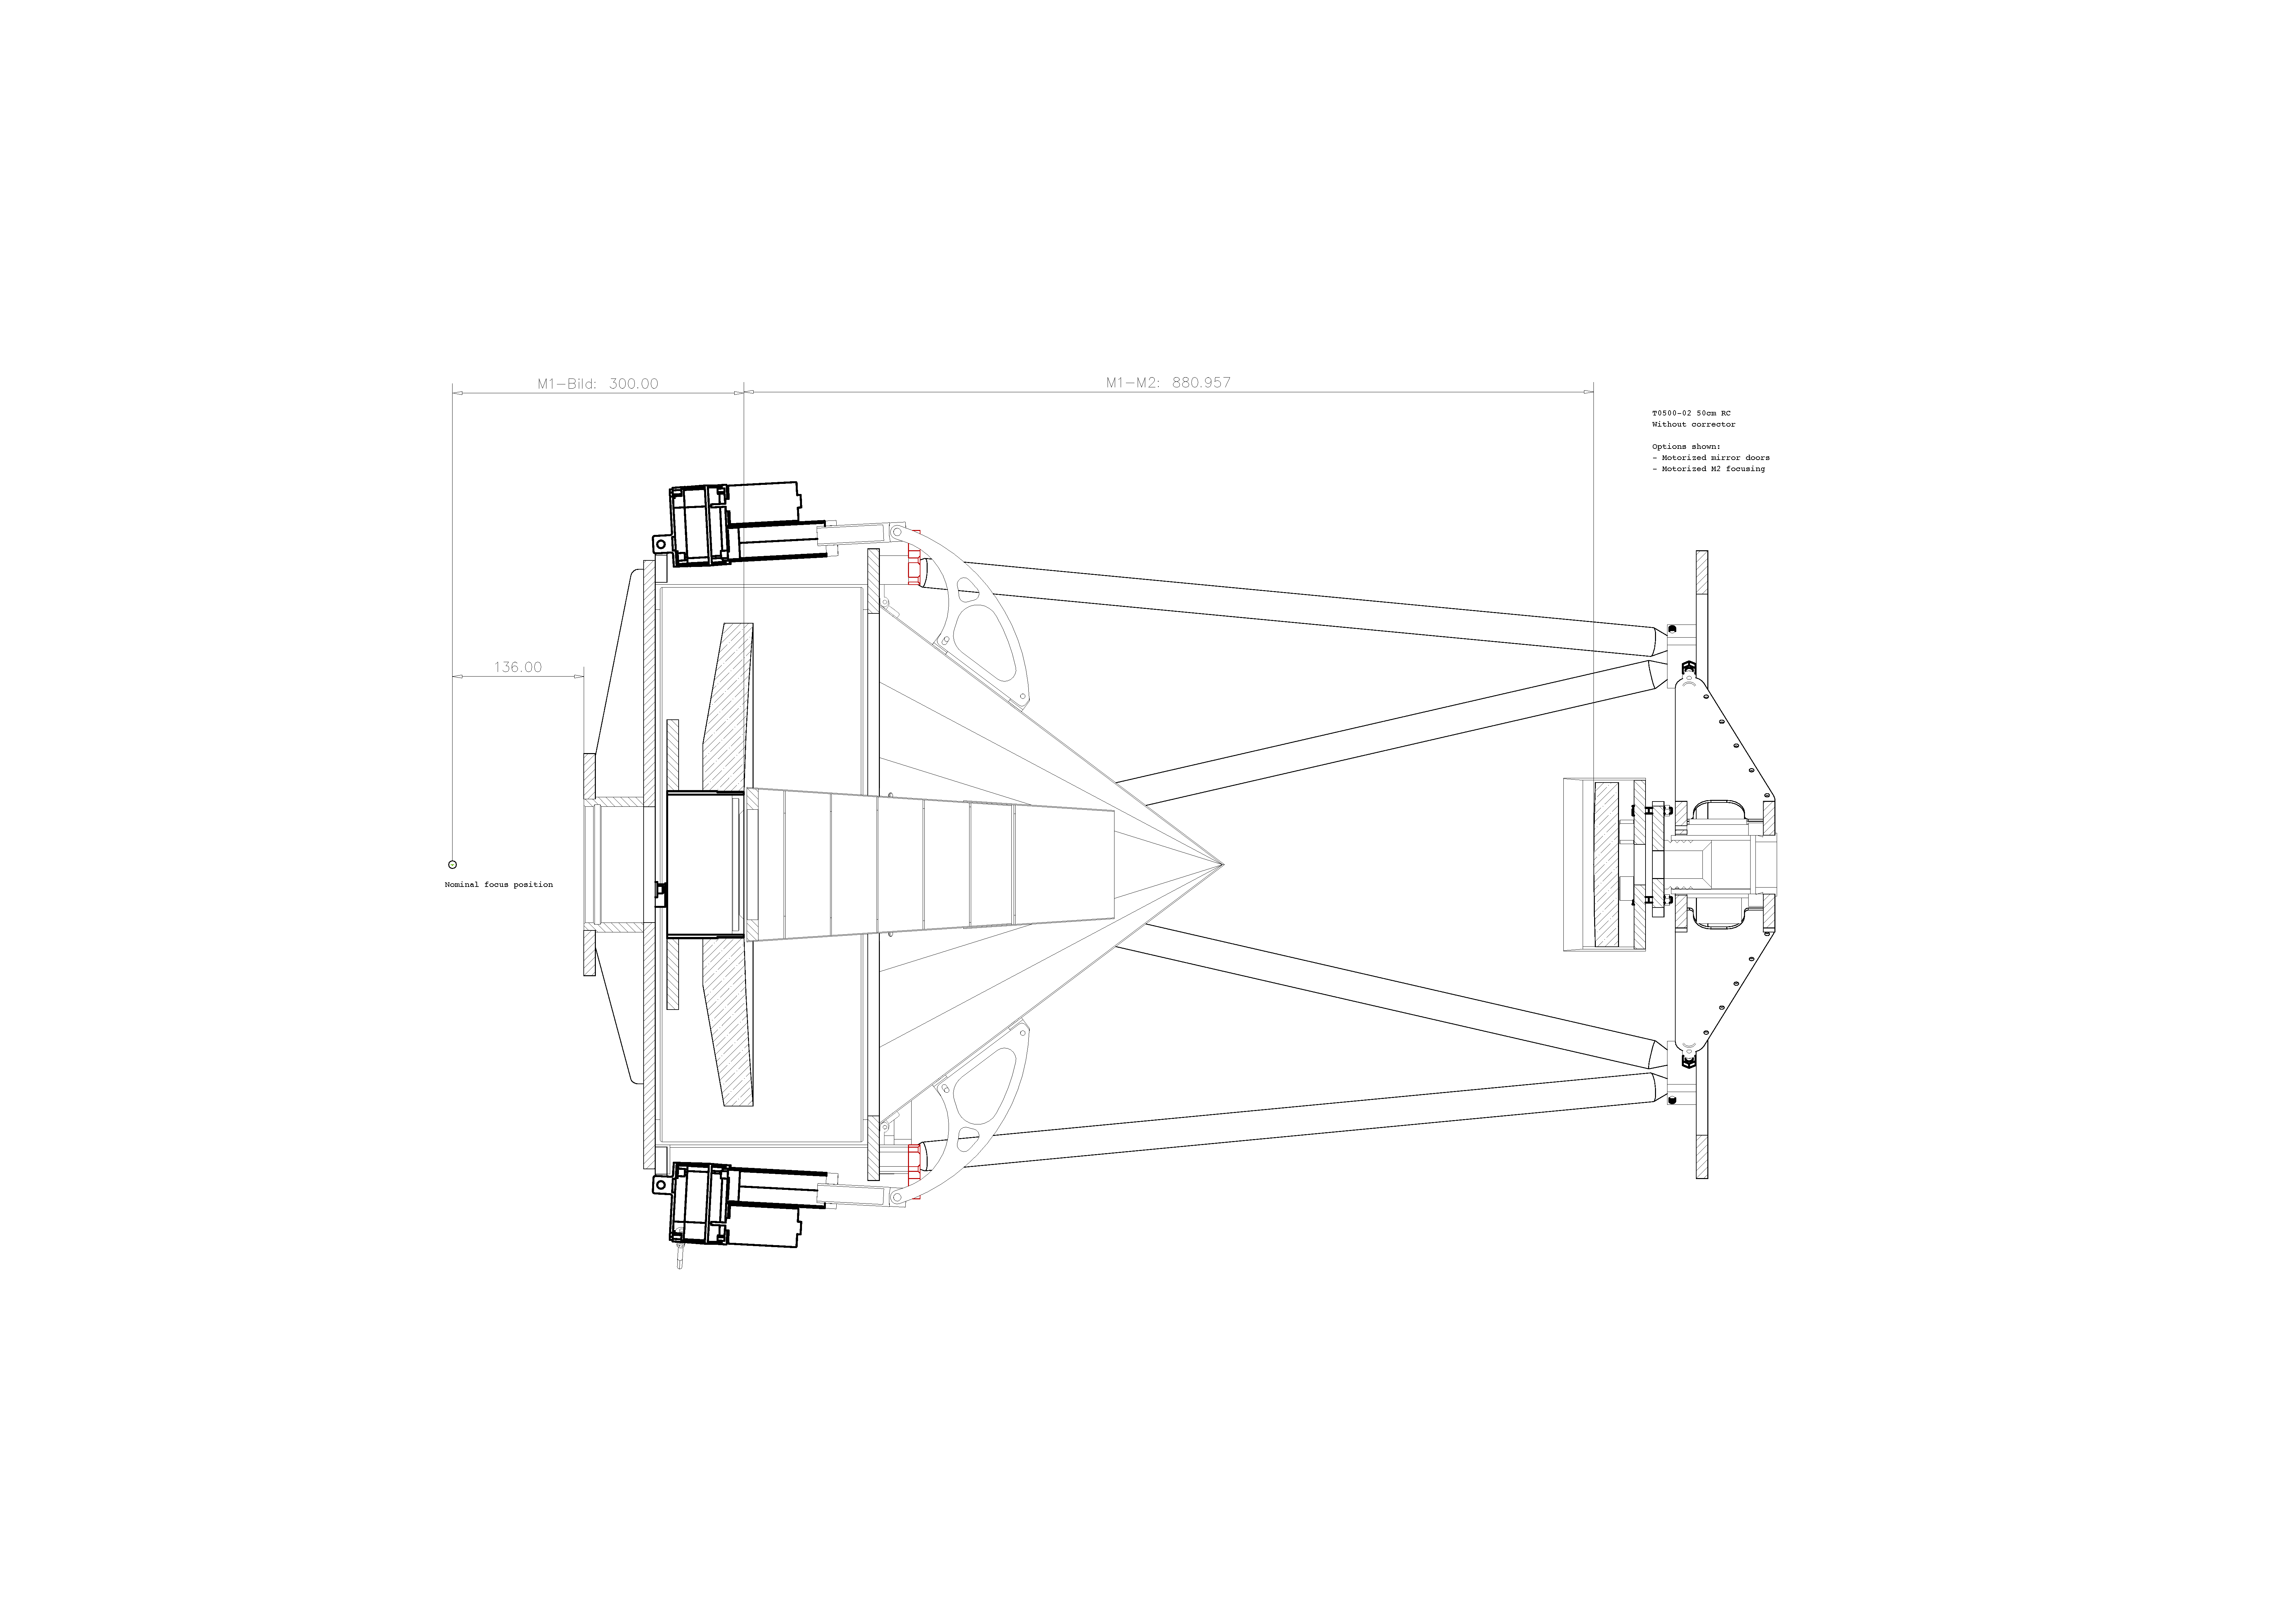
\includegraphics[height=0.9\linewidth,angle=90]{figures/telescope-lateral-section.pdf}
\end{center}
\caption{Lateral section of the telescope. Note that our telescope has a focuser with a different design and that the covers have been removed. The M1 to M2 distance is also different with the 2020 optics.}
\label{figure:telescope-plans-first}
\end{figure}

\begin{figure}
\begin{center}
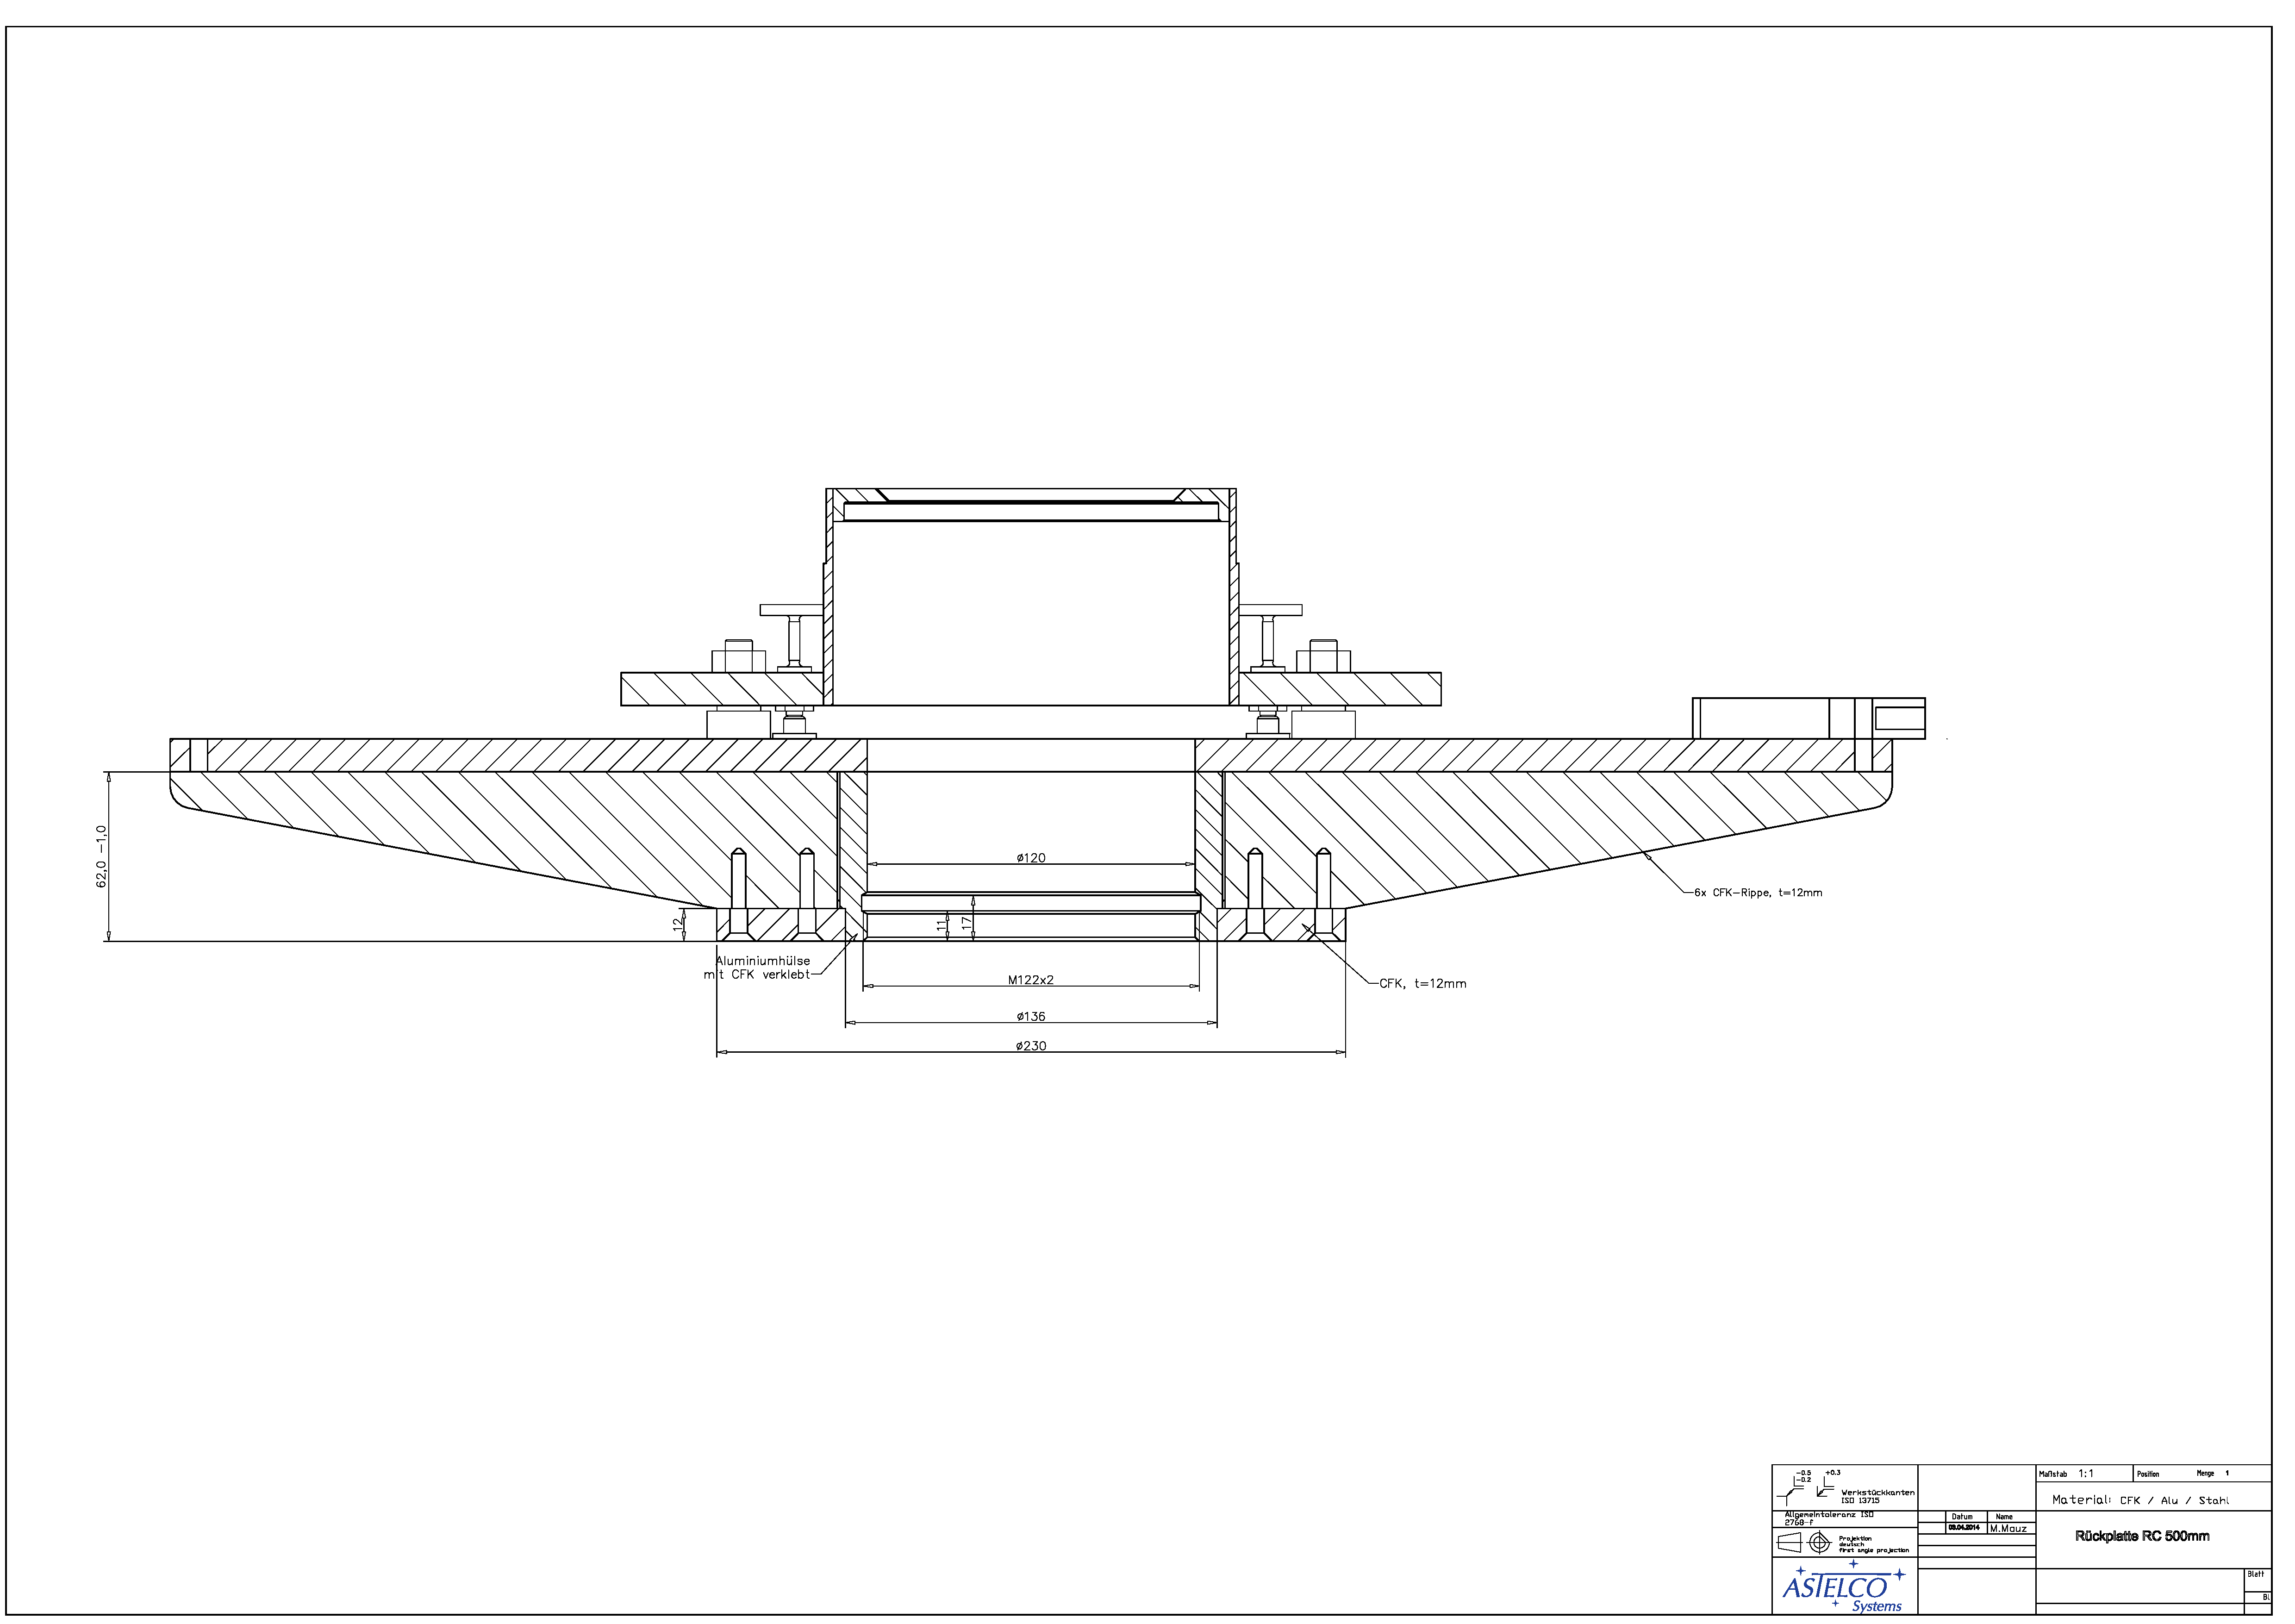
\includegraphics[height=1.0\linewidth,angle=90]{figures/telescope-primary-mirror-cell-backplane-section}
\end{center}
\caption{Lateral section of the backplane of the primary mirror cell.}
\end{figure}

\begin{figure}
\begin{center}
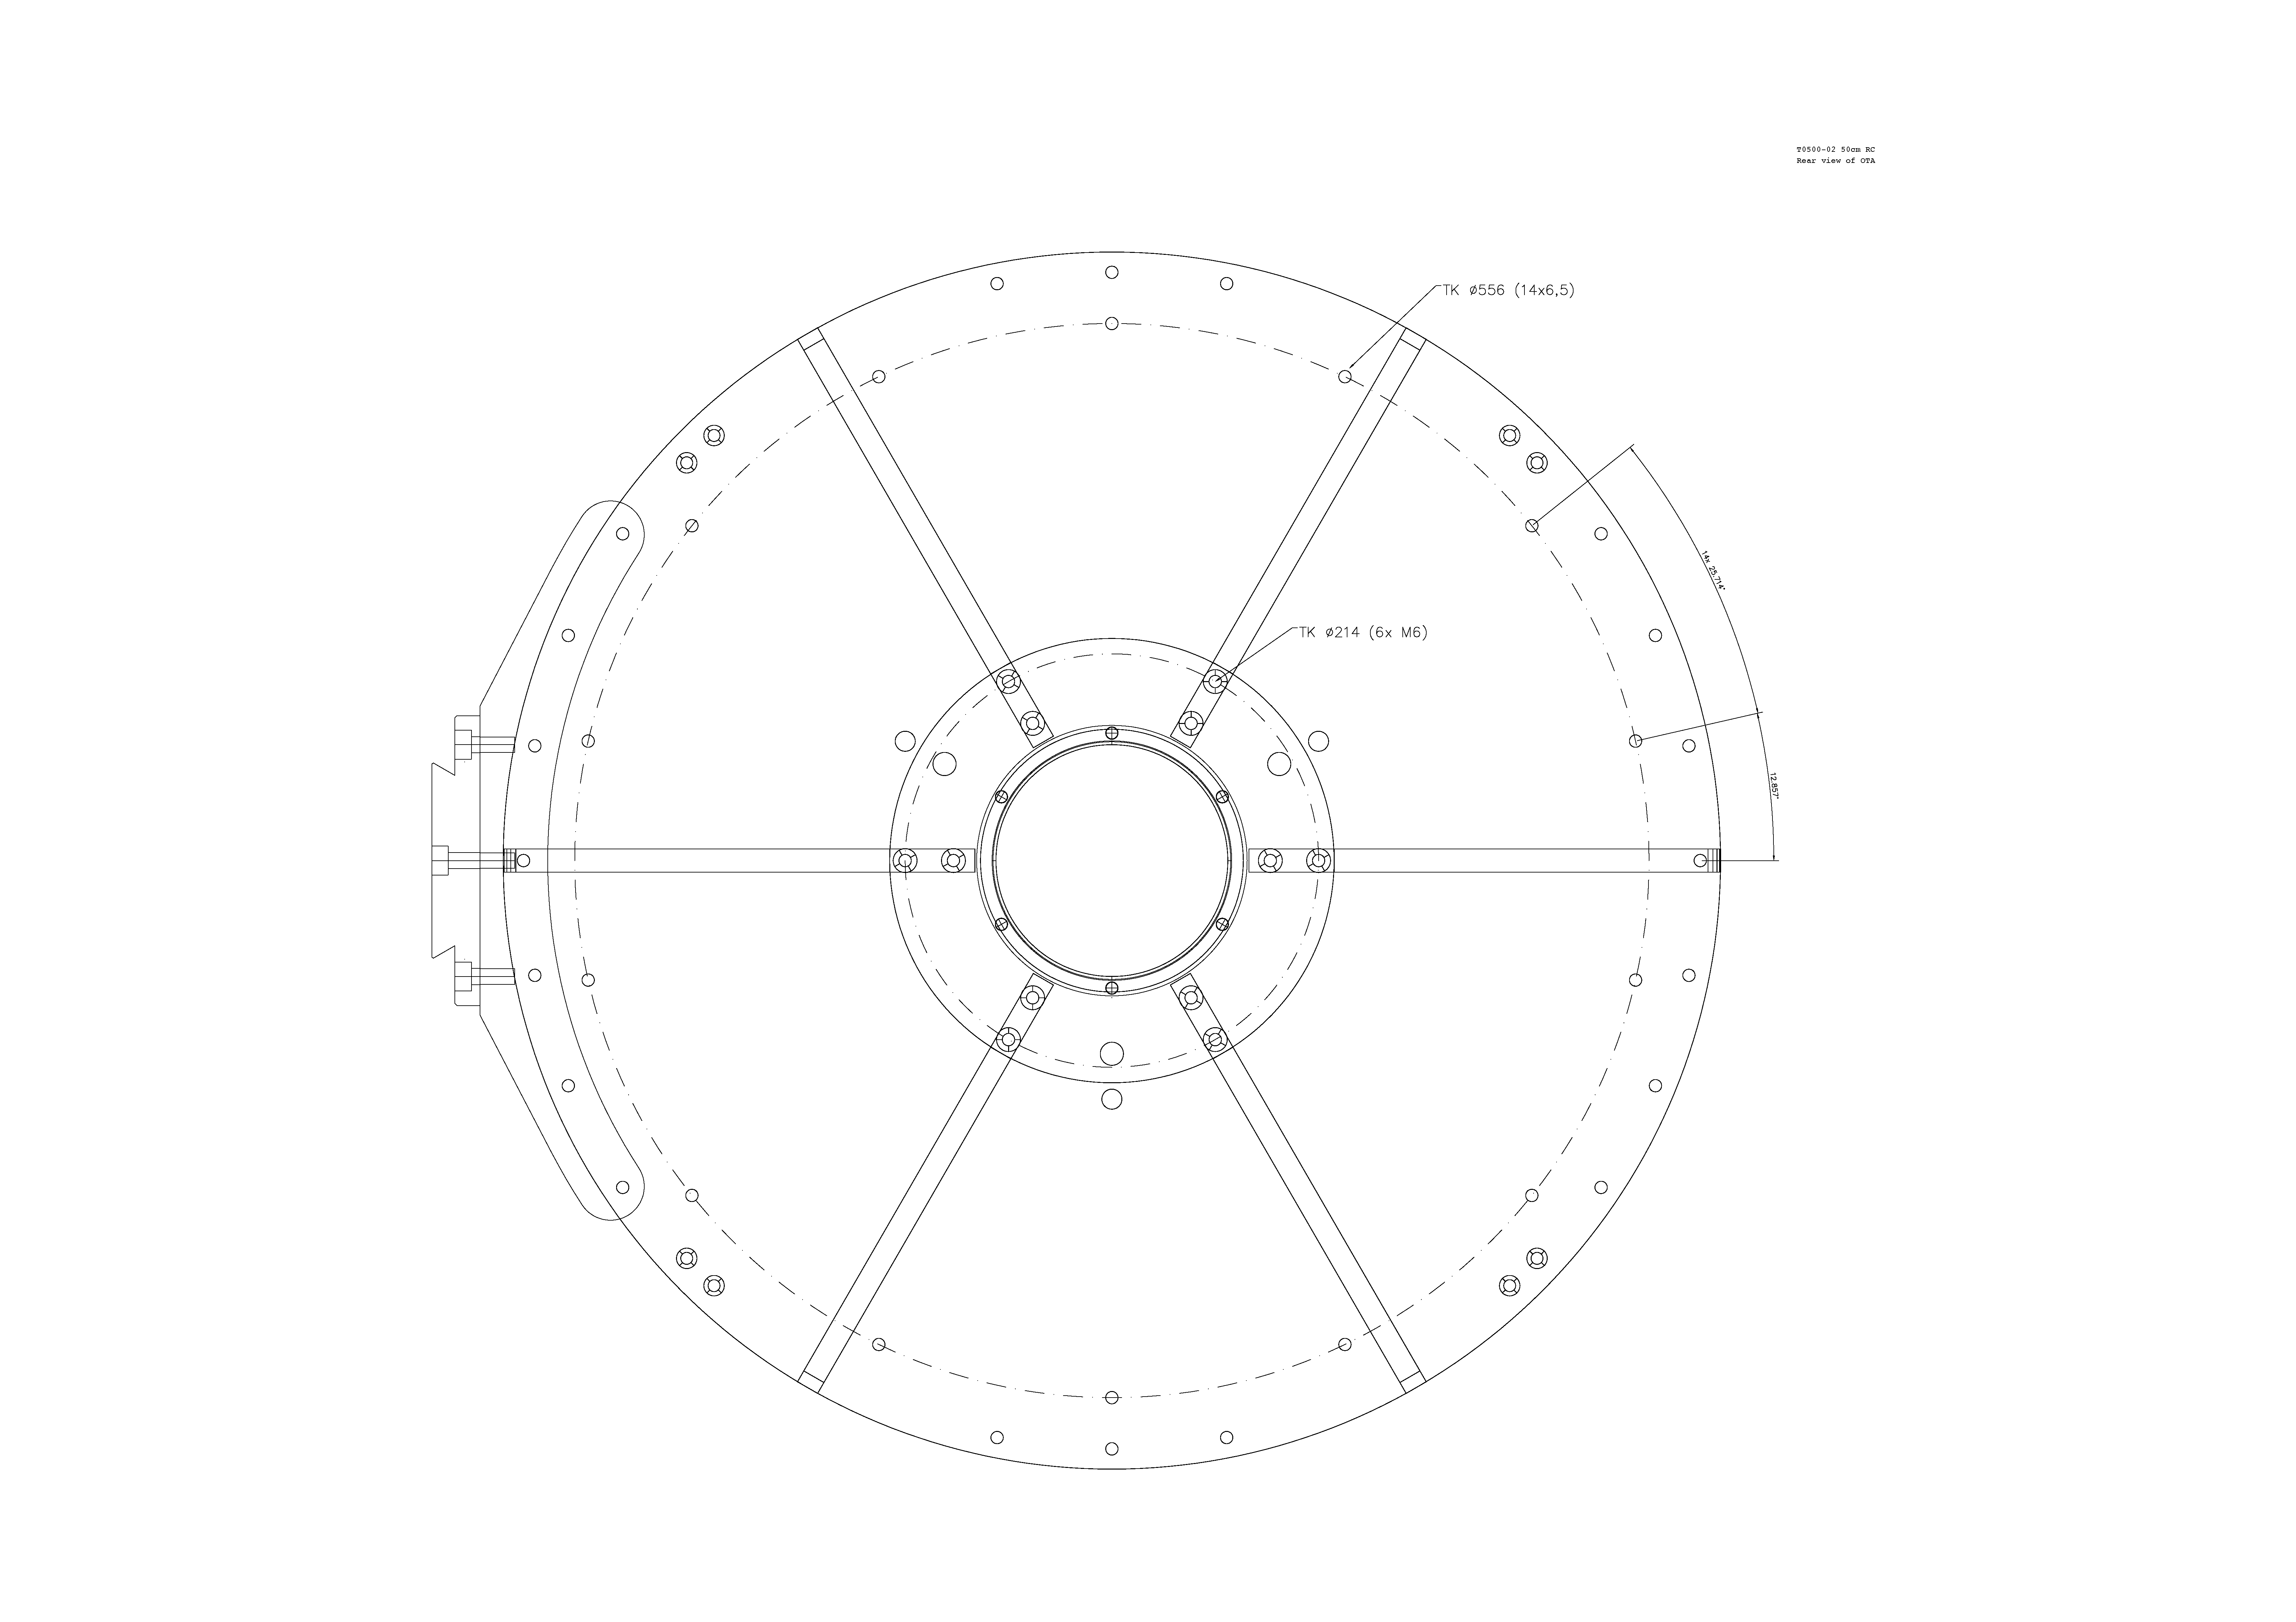
\includegraphics[height=1.0\linewidth,angle=90]{figures/telescope-primary-mirror-cell-rear}
\end{center}
\caption{Lateral section of the telescope.}
\end{figure}

\begin{figure}
\begin{center}
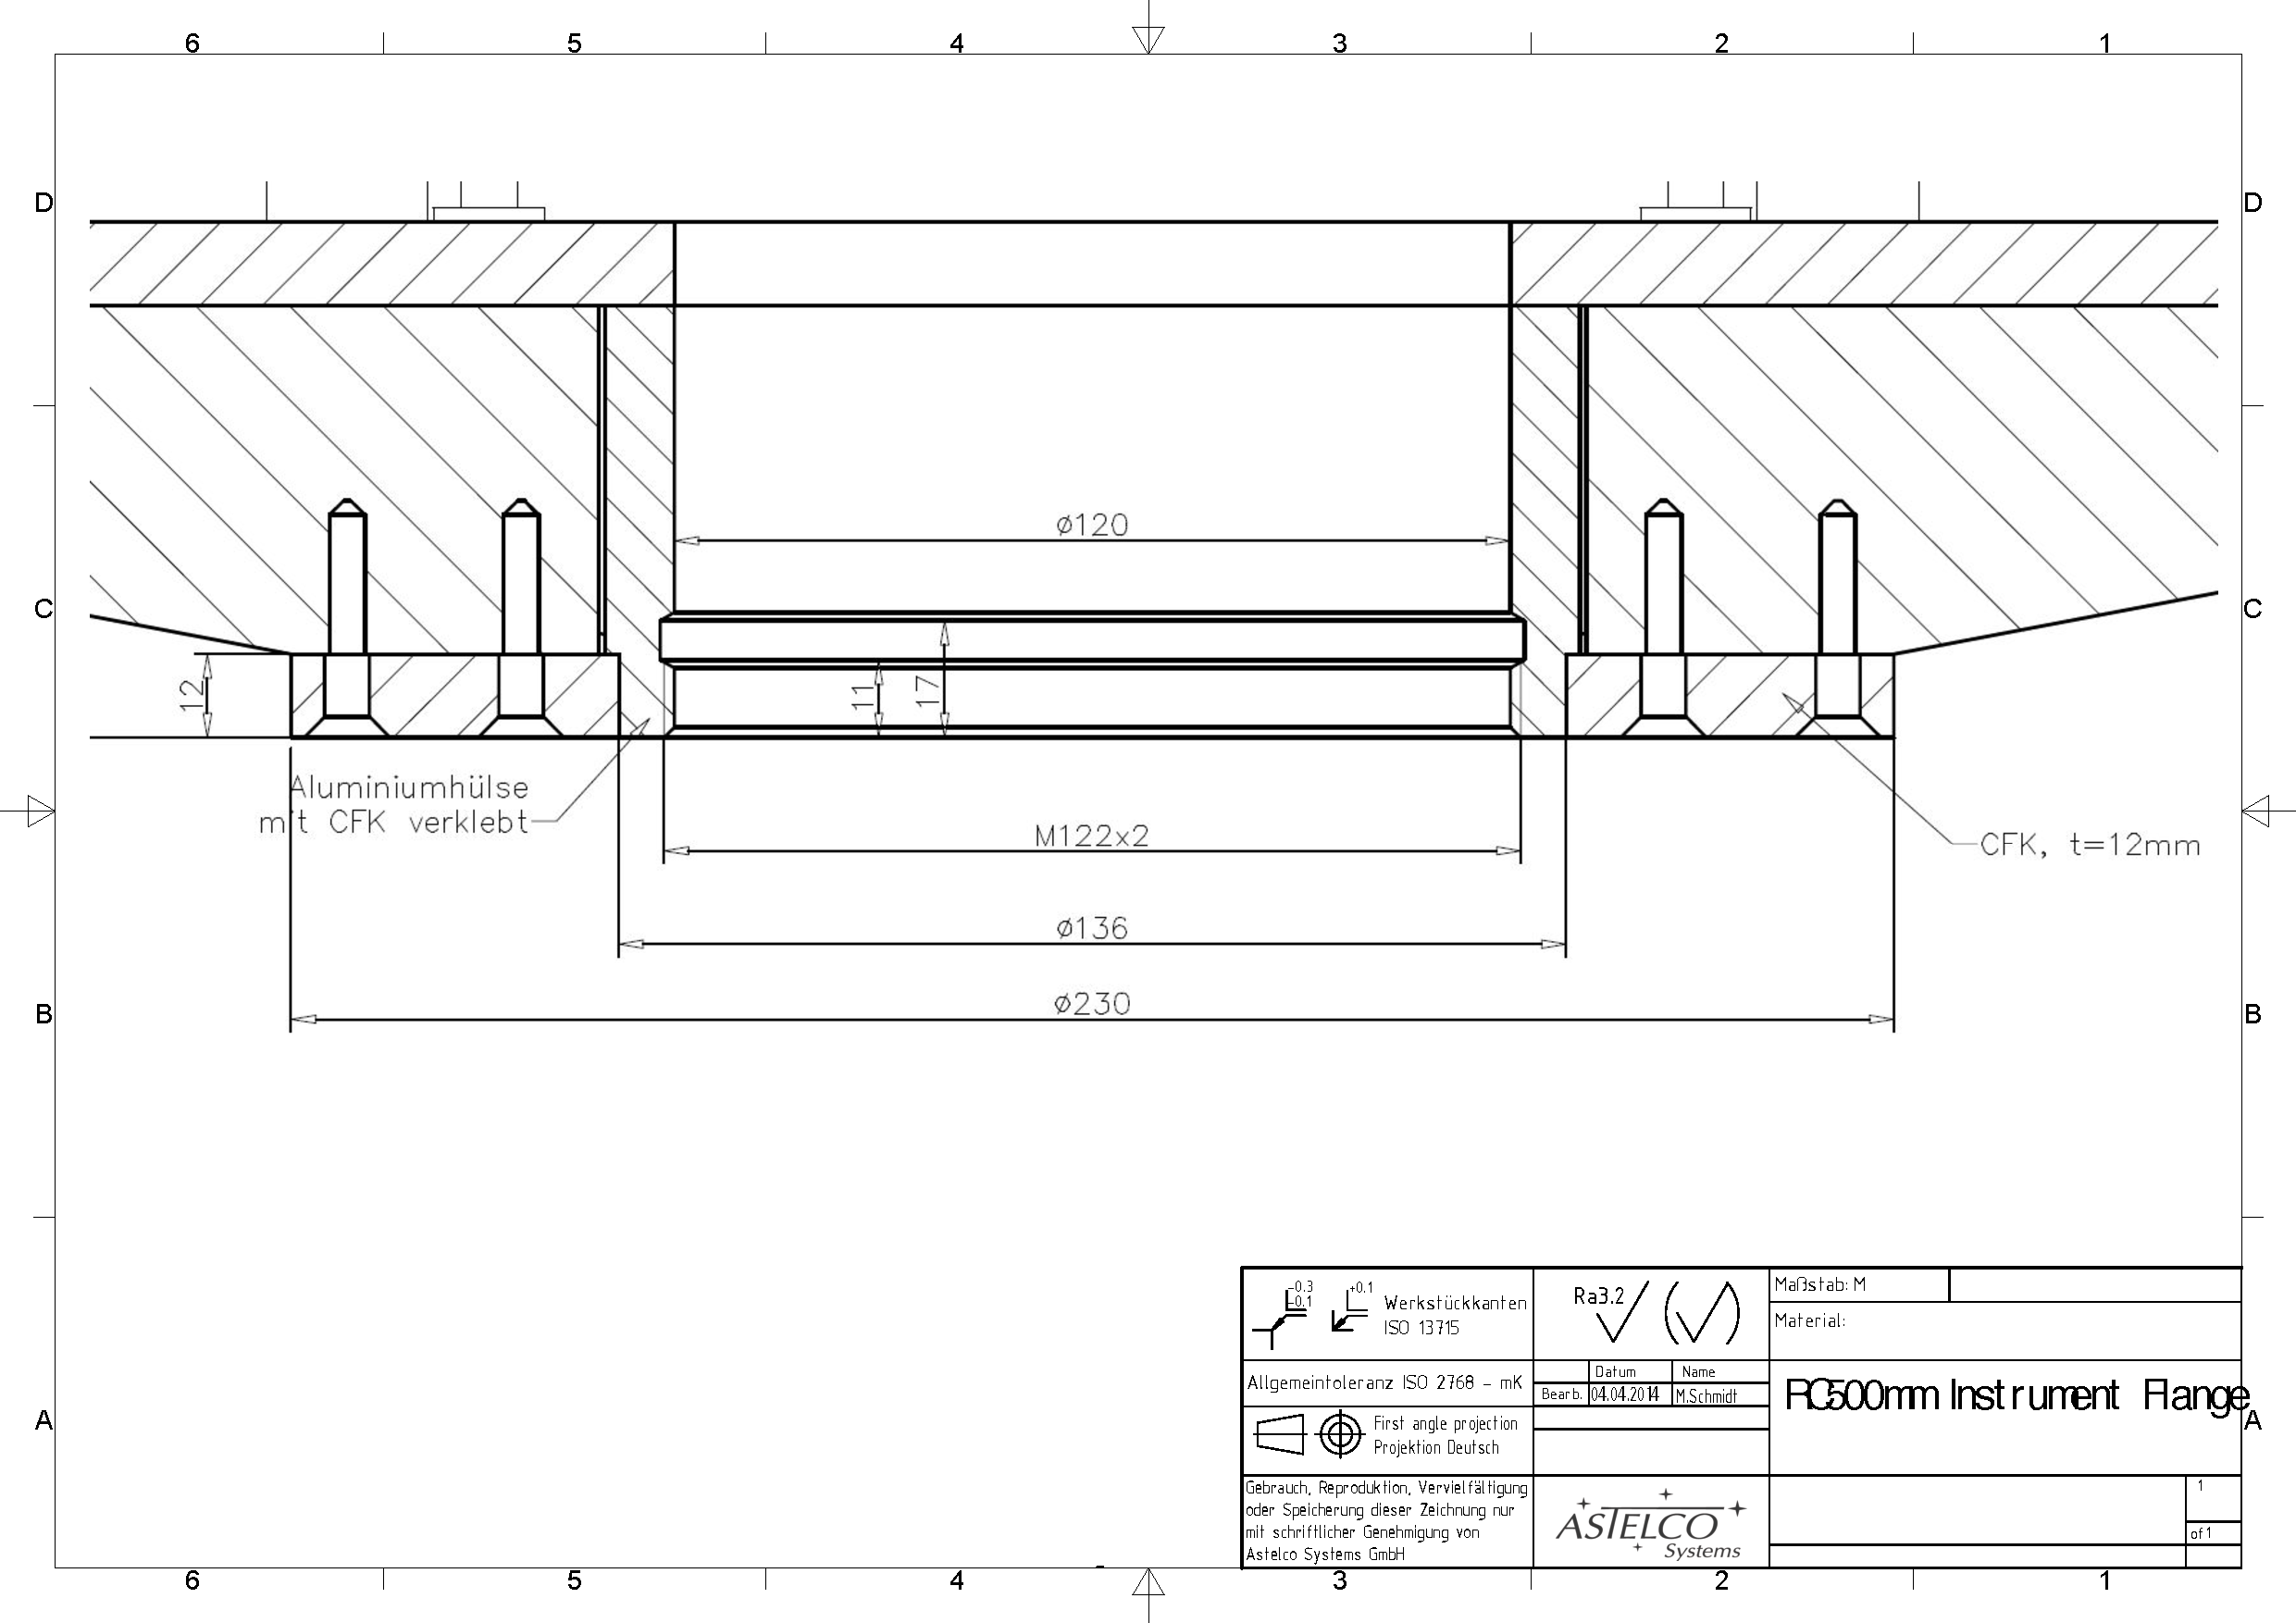
\includegraphics[height=1.0\linewidth,angle=90]{figures/telescope-instrument-flange-section.pdf}
\end{center}
\caption{Lateral section of the instrument flange.}
\label{figure:telescope-plans-last}
\end{figure}



\section{Resumen}

Se presentan los métodos a seguir para retirar o instalar los espejos del telescopio COATLI para su aluninización o servicio de sus componentes.

\section{Descripción general}

COATLI es un telescopio de tipo Ritchey-Chretien de 500 mm de diámetro trabajando en F/8 en una montura ecuatorial de tipo alemán.

El tubo del telescopio, mayormente construido de fibras de carbono tejidas y prensadas, tiene una estructura básica montada sobre el eje de declinación, a la que en adelante se llamará cubo del telescopio o simplemente cubo. En su parte inferior presenta la platina de montaje de instrumentos, en el interior contiene a la celda del primario, que consiste de una placa de soporte y Tip-Tilt. 

En la parte superior del cubo se encuentran las bases de los tubos que forman la estructura Serrurier. Dicha estructura, se completa con el anillo superior, que porta la araña, la araña al sistema de enfoque y éste a la celda del secundario. 

En la base del cubo se encuentran tres tornillos de alineación con tuercas M17 provenientes de la placa de soporte del primario. Entre la placa de soporte y el cubo llevan estos tornillos cada uno un muelle formado por rondanas con forma de menisco. Al lado de éstos tornillos se encuentran tres prisioneros Allen M4 que una vez conseguida la alineación, fijan la placa de soporte del primario.

El bafle del primario pasa a través del boquete central del espejo y se fija en el cubo con tres pares de tornillos similares a los anteriores, tuercas MXX y prisioneros MXX, de manera que su inclinación es independiente de la del espejo primario. Estos tornillos se acceden desde el exterior del cubo, por su agujero central.

La araña se fija en su posición por medio de cuatro tornillos insertados en sendos cilindros, cada uno con una tuerca exterior y otra interior con lo que se puede obtener un descentrado de hasta Nmm del secundario.

La celda del secundario, consiste de una placa sobre la que el espejo va pegado y a la que se fija el bafle mediante tres tornillos radiales. En el bafle, además van montadas tres pestañas de seguridad para el caso de que el secundario se despegase. La alineación se obtiene en forma idéntica a las anteriores, En este caso las tuercas son M10 y los prisioneros MXX

Finalmente, nótese que en la cara sur del estator del eje de AR se encuentra un botón metálico que, al mantenerse presionado, libera los frenos de ambos ejes y es entonces posible mover manualmente el telescopio a las posiciones adecuadas para las operaciones que a continuación se detallarán.

\section{Consideraciones y precauciones generales}

\begin{itemize}
\item Los siguientes procedimientos causarán o bien se iniciarán con un desbalanceo del telescopio en ambos ejes.
\item Recuerde siempre que la única posición relativamente segura en caso de desbalanceo del telescopio, es la de reposo, en la que el eje de AR se encuentra en equilibrio estable y en el eje de Dec. la torca residual es en todo caso muy pequeña.
\item No confie nunca en que los frenos serán capaces de contrarrestar la torca de una posición desbalanceada, se recomienda contar en estos casos , con una tercera persona cuya única función sea la de prevenir una falla de los frenos.
\end{itemize}

\section{Desensamble de la celda del secundario }

\subsection{Requerimientos}

\begin{itemize}
\item Dos personas
\item Llave española M10
\end{itemize}

\subsection{Procedimiento}

\begin{itemize}
\item Presione el botón de liberación de los frenos ubicada en la parte posterior de la montura del telescopio, oriente horizontalmente el tubo del telescopio y libere el botón. 
\item La persona 2 colocará la funda de protección del secundario.
\item La persona 1 extraerá las tuercas M10 y sus rondanas del soporte de la celda, mientras la persona 2 sostiene la celda.
\item La persona 2 extraerá la celda mientras la persona 1 toma las rondanas que forman el muelle.
\item La persona 2 pondrá la celda con el secundario en lugar seguro.
\item Sujetando el tubo y las pesas, presione el botón de liberación de los frenos y regrese el telescopio a la posición de descanso. 
\end{itemize}

\section{Ensamble de la celda del secundario}

\subsection{Requerimientos}

\begin{itemize}
\item Dos personas
\item Llave Allen M5
\end{itemize}

\subsection{Procedimiento}

\begin{itemize}
\item Presione el botón de liberación de los frenos, oriente horizontalmente el tubo del telescopio y libere el botón. 
\item La persona 2 presentará los tornillos de la celda en las cercanías de sus correspondientes boquetes de la placa de montaje.
\item La persona 1 instalará en los tres tornillos, las rondanas que forman los muelles.
\item La persona 1 elegirá la rotación correcta de los tornillos, ya que los prisioneros Allen se accionarán a través de los boquetes que al efecto existen en la placa de montaje.
\item Introdúzcanse los tornillos M10 en sus correspondientes boquetes 
\item La persona 1 se asegurará de que los prisioneros han quedado accesibles y los desenroscará de manera que no entorpezcan el ajuste siguiente. 
\item La persona 2 empujará la celda suavemente, hasta que las rondanas de los muelles entren en contacto con la celda y la placa.
\item La persona 1 instalará las tuercas M10 y sus rondanas de soporte de la celda, apretándolas a mano.
\item La persona 1 aplicará una precarga mediante dos vueltas de las tuercas usando la llave española M10
\item La persona 1 ajustará los prisioneros Allen para fijar la celda en esa posición.
\item Presione el botón de liberación de los frenos y lleve el telescopio a la posición de reposo.
\end{itemize}

\section{Desensamble del Bafle del primario}

\subsection{Requerimientos}

\begin{itemize}
\item Dos personas
\item Llave española Mxx
\item Llave Allen MXX
\end{itemize}

\subsection{Procedimiento}

\begin{itemize}
\item Abra las tapas de protección del primario. 
\item Presione el botón de liberación de los frenos, oriente horizontalmente el tubo del telescopio y libere el botón. 
\item La persona 2 sujetará el bafle usando guantes de látex, permitiendo las oscilaciones que se producirán, pero manteniendo una ligera presión hacia la celda
\item La persona 1 localizará las tuercas MXX de soporte y alineación del bafle dentro del boquete del Cubo y procederá a extraerlas con sus rondanas de forma pareja, para limitar las oscilaciones del bafle.
\item La persona 2 extraerá el bafle mientras la persona 1 vigila las rondanas que forman el muelle, mismas que no deberían salirse de los tornillos gracias a un arosello que debe impedirlo.
\item La persona 2 colocará el bafle en lugar seguro y protegido.
\item Cierre las tapas de protección del primario.
\item Presione el botón de liberación de los frenos y regrese a la posición de reposo.
\end{itemize}

\section{Ensamble del Bafle del primario}

\subsection{Requerimientos}

\begin{itemize}
\item Dos personas
\item Llave española Mxx
\item Llave Allen MXX
\end{itemize}

\subsection{Procedimiento}

\begin{itemize}
\item Abra las tapas de protección del primario. 
\item Presione el botón de liberación de los frenos, oriente horizontalmente el tubo del telescopio y libere el botón. 
\item La persona 2 usando guantes de látex, introducirá el bafle por el boquete del primario, girándolo según las instrucciones que le dará la persona 1 para hacer coincidir los tornillos con las perforaciones correspondientes. 
\item La persona 1 insertará las tuercas MXX de soporte y alineación del bafle dentro del boquete del Cubo y procederá a atornillarlas a mano. 
\item La persona 1 aplicará una precarga a las tuercas girándolas dos vueltas
\item Cierre las tapas de protección del primario.
\end{itemize}

\section{Desensamble de la celda del primario}

Si se encuentra instalado algún instrumento en la celda del primario, desinstálelo siguiendo el procedimiento recomendado para dicho instrumento.
Si el Bafle del primario está instalado, siga el correspondiente procedimiento de desinstalación. 

\subsection{Requerimientos}

\begin{itemize}
\item Dos personas
\item Llave española M17
\item Llave Allen MXX 
\item Guantes de látex
\end{itemize}

\subsection{Procedimiento}

\begin{itemize}
\item Abra las tapas de protección del primario. Puede ser necesario retirar alguno?
\item Presione el botón de liberación de los frenos, oriente el tubo del telescopio hacia el cenit y libere el botón. 
\item La persona 1 localizará las tuercas M17 de soporte y alineación del primario en la parte inferior del Cubo y procederá a extraerlas con sus rondanas de forma pareja, para limitar las oscilaciones del primario.
\item La persona 2, con guantes de látex extraerá el primario con su celda sujetándolo a través del boquete del primario.
\item Mientras tanto, la persona 1 vigilará las rondanas que forman el muelle, mismas que no deberían salirse de los tornillos gracias a un arosello que debe impedirlo.
\item La persona 2 colocará el primario con su celda en lugar seguro y protegido. Esto puede requerir mas aclaraciones
\item Presione el botón de liberación de los frenos y regrese a la posición de reposo.
\end{itemize}

\section{Ensamble de la celda del primario}

\subsection{Requerimientos}

\begin{itemize}
\item Dos personas
\item Llave española M17
\item Llave Allen MXX
\item Guantes de látex
\end{itemize}

\subsection{Procedimiento}

\begin{itemize}
\item Abra las tapas de protección del primario. Puede ser necesario retirar alguno?
\item Presione el botón de liberación de los frenos, oriente el tubo del telescopio hacia el cenit y libere el botón. 
\item La persona 2, con guantes de látex sujetando la celda a través del boquete del primario presentará, los tornillos de la celda en las cercanías de sus correspondientes boquetes en el Cubo.
\item La persona 1 indicará a la 2 la rotación correcta de la celda para los siguientes pasos
\item La persona 1 vigilará las rondanas que forman el muelle, mismas que no deberían salirse de los tornillos gracias a un arosello que debe impedirlo.
\item Introdúzcanse los tornillos Mxx en sus correspondientes boquetes 
\item La persona 1 desatornillará los prisioneros de fijación de la celda, de manera que no entorpezcan el ajuste siguiente. 
\item La persona 1 atornillará las tuercas M17 de soporte y alineación del primario en la parte inferior del Cubo apretándolas a mano.
\item La persona 1 aplicara una precarga a las tuercas usando la llave española M17, dándole dos vueltas a cada una.
\item La persona 1 ajustará los prisioneros Mxx 
\item Presione el botón de liberación de los frenos y regrese a la posición de reposo.
\end{itemize}

\section{Notas}

\begin{itemize}
\item Ya que la inclinación del bafle del primario es independiente de la alineación del espejo, es necesario contar con un método para alinearlo. Se sugiere usar hilos cruzados desde los tubos Serrurier, formando una cruz a la altura de la entrada del bafle y ya que la exactitud de la posición de dicha retícula puede ser engañosa por causa de la inclinación de los tubos, incertidumbres en la alineación del láser y posibles asimetrías, se puede verificar su centrado observando el paso del láser, una vez alineado con el secundario, usando un papel sobre la misma retícula. Si fuese necesario, se pueden modificar los hilos para señalar el nuevo punto de referencia para realinear el bafle con ese punto, para lo que sería necesario abrir el acceso a los tornillos en la base del bafle.   
\item Es conveniente fabricar una cubierta para el primario para protegerlo durante las manipulaciones.
\item La funda del bafle del secundario ajusta demasiado, se recomienda aumentar su diámetro y añadirle un resorte para facilitar su instalación. 
\end{itemize}

\section{Recoating}

ASTELCO recommend removing the aluminum and MgF$_2$ coatings by soaking in a 10\% solution of NaOH for several hours.


\section{Preguntas}

¿Cuáles son las constantes cónicas medidas de los espejos?

¿En qué material están construidos?

¿Las películas de Al tienen capas protectoras? Y de ser así, ¿Qué procedimiento debe seguirse para retirarlas?

Una vez retirado el bafle y las tuercas de los tornillos de jalar del primario, para retirarlo del telescopio:

¿El espejo y su base caben entre las barras del serrurier o es necesario desmontar antes algo más?

 ¿Es necesario para aluminizar, despegar el primario y/o el secundario de las placas de carbón que los portan?, de ser así, ¿Cuáles son los procedimientos necesarios para hacerlo y posteriormente para pegarlo?

¿Cuál es el cemento con el que está pegado? ¿Cuál es su expectativa de vida?

En ambas celdas, ¿Qué es lo que evita que los tornillos de jalar giren? Y ¿Sobre qué apoyan los tornillos de empujar?

\section{Hartmann Test}

\begin{figure*}
\begin{center}
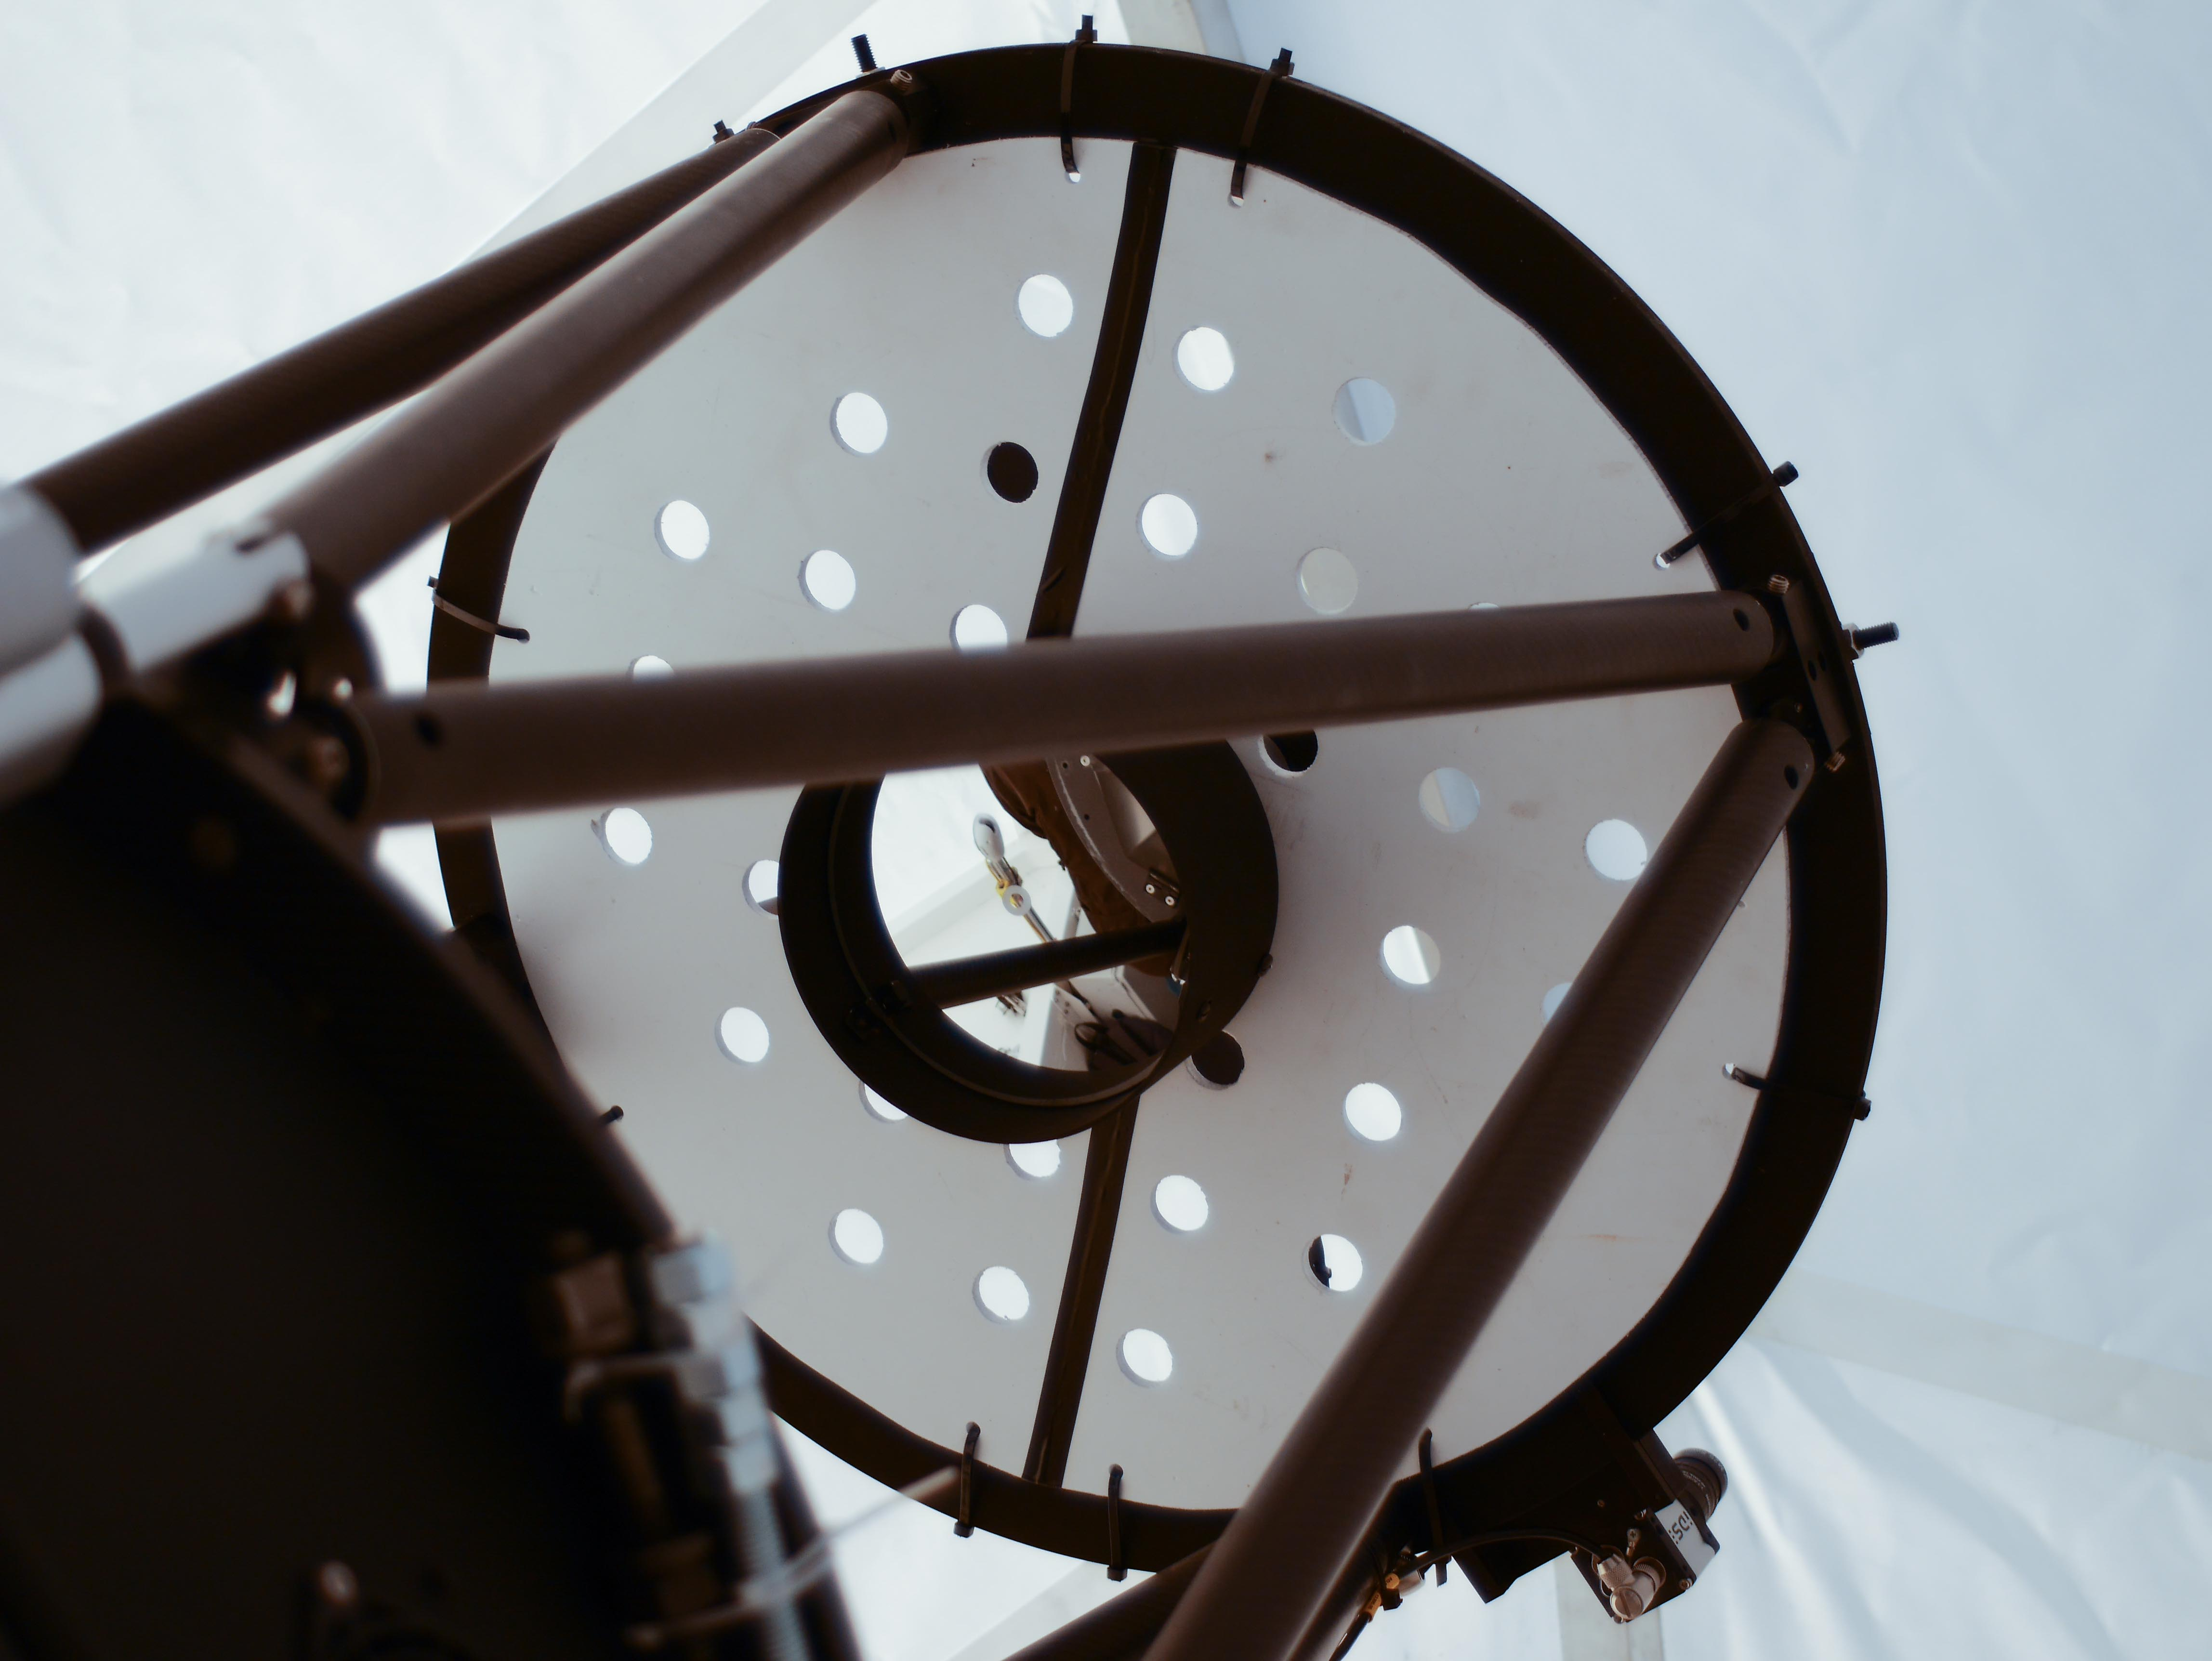
\includegraphics[width=1.0\linewidth]{figures/telescope-hartmann-mask-mounted.jpg}
\end{center}
\caption{The Hartmann mask mounted on the telescope..}
\label{figure:telescope-hartmann-mask-mounted}
\end{figure*}

\begin{figure*}
\begin{center}
\resizebox{\columnwidth}{!}{
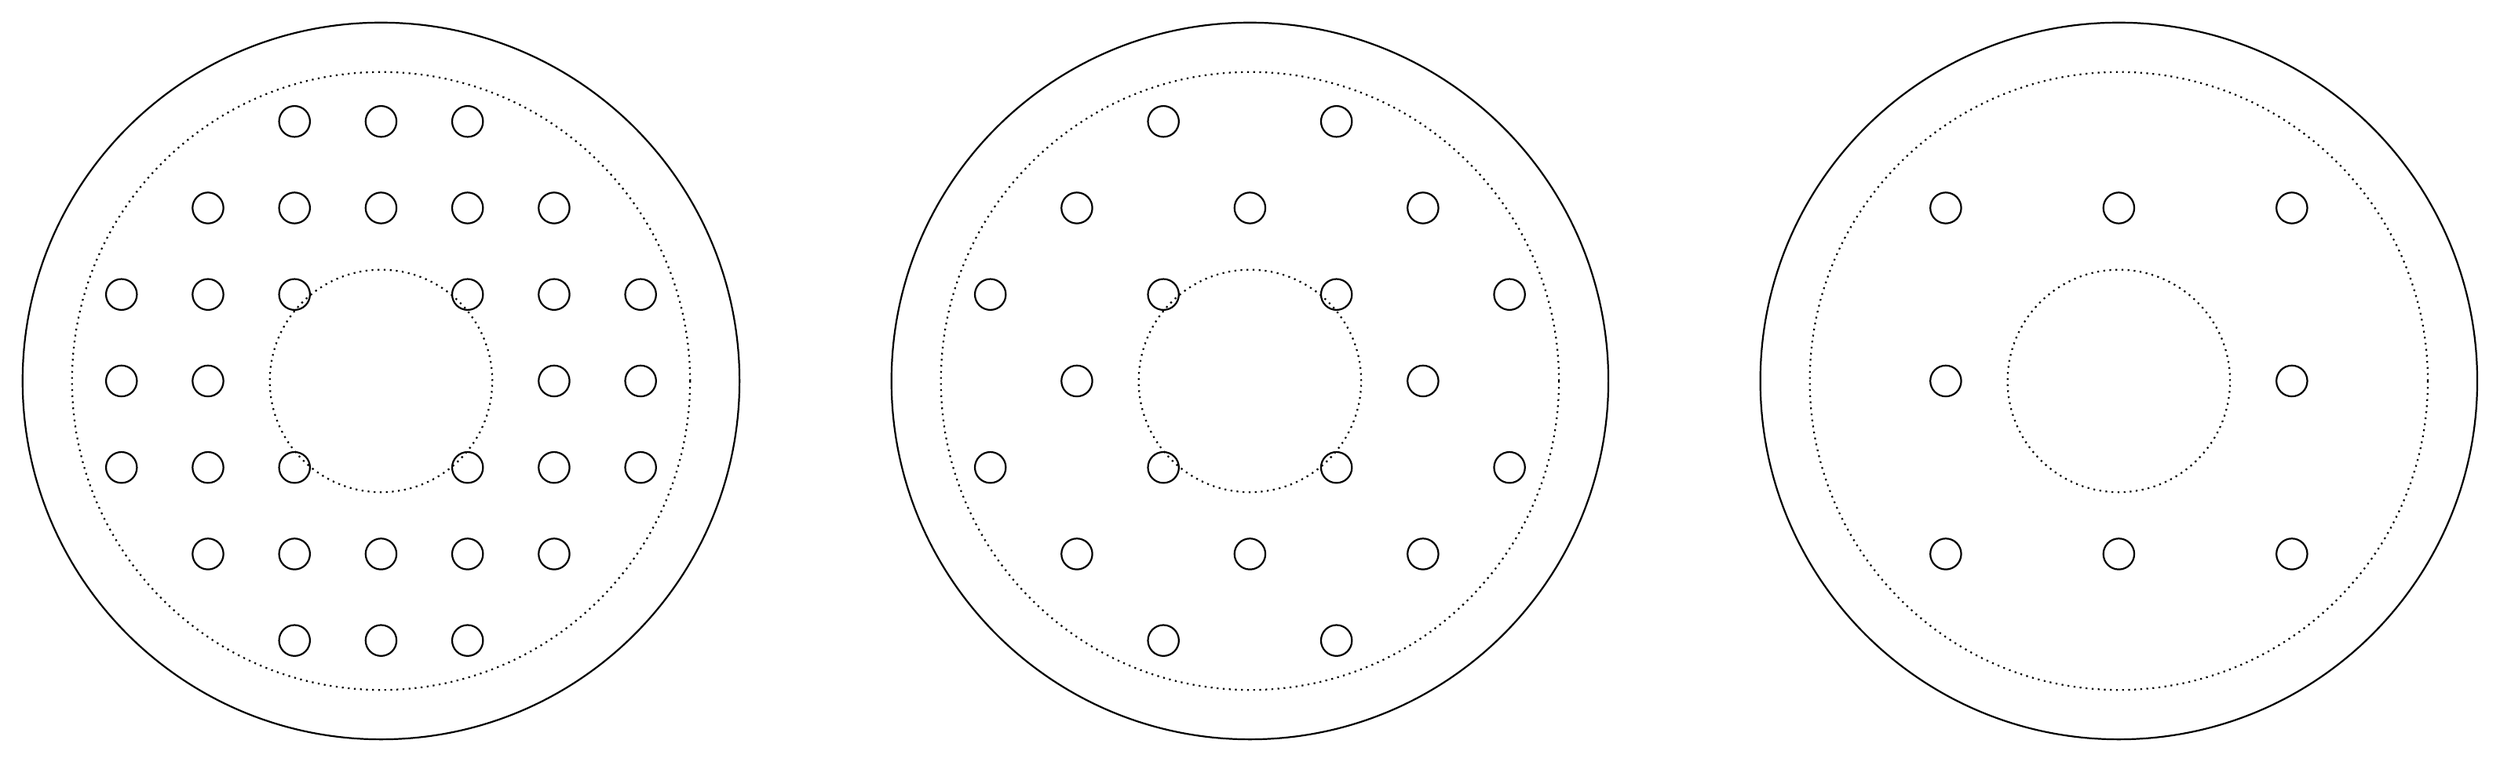
\begin{tikzpicture}[
 scale=0.2,
 thick
]
\begin{scope}[xshift=0,yshift=0]
\draw (0,0) circle (29);
\draw (+7,+7) circle (1.25);
\draw (+7,-7) circle (1.25);
\draw (-7,+7) circle (1.25);
\draw (-7,-7) circle (1.25);
\draw (0,+14) circle (1.25);
\draw (0,-14) circle (1.25);
\draw (+14,0) circle (1.25);
\draw (-14,0) circle (1.25);
\draw (+7,+14) circle (1.25);
\draw (-7,+14) circle (1.25);
\draw (+7,-14) circle (1.25);
\draw (-7,-14) circle (1.25);
\draw (+14,+7) circle (1.25);
\draw (+14,-7) circle (1.25);
\draw (-14,+7) circle (1.25);
\draw (-14,-7) circle (1.25);
\draw (+14,+14) circle (1.25);
\draw (+14,-14) circle (1.25);
\draw (-14,+14) circle (1.25);
\draw (-14,-14) circle (1.25);
\draw (-21,+7) circle (1.25);
\draw (-21,0) circle (1.25);
\draw (-21,-7) circle (1.25);
\draw (+21,+7) circle (1.25);
\draw (+21,0) circle (1.25);
\draw (+21,-7) circle (1.25);
\draw (+7,+21) circle (1.25);
\draw (0,+21) circle (1.25);
\draw (-7,+21) circle (1.25);
\draw (+7,-21) circle (1.25);
\draw (0,-21) circle (1.25);
\draw (-7,-21) circle (1.25);
\draw (0,0) [dotted] circle (25);
\draw (0,0) [dotted] circle (9);
\end{scope}
\begin{scope}[xshift=2000,yshift=0]
\draw (0,0) circle (29);
\draw (+7,+7) circle (1.25);
\draw (+7,-7) circle (1.25);
\draw (-7,+7) circle (1.25);
\draw (-7,-7) circle (1.25);
\draw (0,+14) circle (1.25);
\draw (0,-14) circle (1.25);
\draw (+14,0) circle (1.25);
\draw (-14,0) circle (1.25);
%\draw (+7,+14) circle (1.25);
%\draw (-7,+14) circle (1.25);
%\draw (+7,-14) circle (1.25);
%\draw (-7,-14) circle (1.25);
%\draw (+14,+7) circle (1.25);
%\draw (+14,-7) circle (1.25);
%\draw (-14,+7) circle (1.25);
%\draw (-14,-7) circle (1.25);
\draw (+14,+14) circle (1.25);
\draw (+14,-14) circle (1.25);
\draw (-14,+14) circle (1.25);
\draw (-14,-14) circle (1.25);
\draw (-21,+7) circle (1.25);
%\draw (-21,0) circle (1.25);
\draw (-21,-7) circle (1.25);
\draw (+21,+7) circle (1.25);
%\draw (+21,0) circle (1.25);
\draw (+21,-7) circle (1.25);
\draw (+7,+21) circle (1.25);
%\draw (0,+21) circle (1.25);
\draw (-7,+21) circle (1.25);
\draw (+7,-21) circle (1.25);
%\draw (0,-21) circle (1.25);
\draw (-7,-21) circle (1.25);
\draw (0,0) [dotted] circle (25);
\draw (0,0) [dotted] circle (9);
\end{scope}
\begin{scope}[xshift=4000,yshift=0]
\draw (0,0) circle (29);
%\draw (+7,+7) circle (1.25);
%\draw (+7,-7) circle (1.25);
%\draw (-7,+7) circle (1.25);
%\draw (-7,-7) circle (1.25);
\draw (0,+14) circle (1.25);
\draw (0,-14) circle (1.25);
\draw (+14,0) circle (1.25);
\draw (-14,0) circle (1.25);
%\draw (+7,+14) circle (1.25);
%\draw (-7,+14) circle (1.25);
%\draw (+7,-14) circle (1.25);
%\draw (-7,-14) circle (1.25);
%\draw (+14,+7) circle (1.25);
%\draw (+14,-7) circle (1.25);
%\draw (-14,+7) circle (1.25);
%\draw (-14,-7) circle (1.25);
\draw (+14,+14) circle (1.25);
\draw (+14,-14) circle (1.25);
\draw (-14,+14) circle (1.25);
\draw (-14,-14) circle (1.25);
%\draw (-21,+7) circle (1.25);
%\draw (-21,0) circle (1.25);
%\draw (-21,-7) circle (1.25);
%\draw (+21,+7) circle (1.25);
%\draw (+21,0) circle (1.25);
%\draw (+21,-7) circle (1.25);
%\draw (+7,+21) circle (1.25);
%\draw (0,+21) circle (1.25);
%\draw (-7,+21) circle (1.25);
%\draw (+7,-21) circle (1.25);
%\draw (0,-21) circle (1.25);
%\draw (-7,-21) circle (1.25);
\draw (0,0) [dotted] circle (25);
\draw (0,0) [dotted] circle (9);
\end{scope}
\end{tikzpicture}
}
\end{center}
\caption{The geometry of the Hartmann mask. The raw grid spacing is 70 mm (left). By covering holds with tape, this can be used to create less dense grids with spacings of 100 mm (center) and 140 mm (right).}
\label{figure:telescope-hartmann-mask-geometry}
\end{figure*}

We have constructed a Hartmann mask for the telescope. The mask has an array of 25 mm diameter holes on a Cartesian grid with a spacing of 70 mm between hole centers. By blocking holes with tape, one can create grids with spacings of 70, 100, and 140 mm (see Figure~\ref{figure:telescope-hartmann-mask-geometry}).

The mask is split into two to facilitate mounting. It should be secured to the secondary ring with cable ties and the joints between the two sections should be covered with tape. The telescope needs rebalancing in both axes after mounting the mask.

\subsection{Spherical Aberration}

In a conventional Hartmann test, one moves the detector and leaves the optical system fixed. However, this is not convenient here and we instead will move the secondary and leave the detector fixed. This will introduce spherical aberration. We have quantified this in ZEMAX using the nominal telescope design.

We placed a grid of rays on the pupil and then measured the radii $R_\mathrm{outer}$ and $R_\mathrm{inner}$ of the innermost and outermost points in the intrafocal and extrafocal images as function of the distance between M1 and M2. We interpolate the outer radii to zero to define the position of best focus. We then interpolate the inner radii to the same position determine the radius $R_\mathrm{inner}^\mathrm{best}$ of the image formed by the inner part of the pupil. We see that for images taken with the secondary moved $\pm1.0$, the spherical aberration amounts to 0.4 {\micron} or 0.02 arcsec radius in the interpolated best image plane. For images taken with the secondary moved $\pm1.5$, this rises to 2.0 {\micron} or 0.10 arcsec radius. 

The diffraction-limited image radius for the telescope in $B$ is $\lambda f/2D$ or about 1.8 {\micron} or 0.09 arcsec. Thus, for $\pm1.5$ mm displacement of the secondary, the spurious spherical aberration is small compared to the seeing but comparable to the diffraction limit and for $\pm 1.0$ mm displacement of the secondary, the spurious spherical aberration is small even compared to the diffraction limit. These should be borne in mind when determining the appropriate secondary displacement to use for a given application of the Hartmann test.

\begin{table}
\caption{Spherical Aberration in the Hartmann Test}
\label{table:hartmann-spherical-aberration}
\begin{center}
\begin{tabular}{ccccc}
\hline
\hline
$M1-M2$&$\Delta(M1-M2)$&$R_\mathrm{outer}$&$R_\mathrm{inner}$&$R_\mathrm{inner}^\mathrm{best}$\\
(mm)&(mm)&(\micron)&(\micron)&(\micron)\\
\hline
880.457&$-0.5$&343.3720&116.5\\
881.457&$+0.5$&343.372&117.2\\
&&&&0.7\\
\hline
879.957&$-1.0$&689.912&233.2\\
881.957&$+1.0$&688.212&234.1\\
&&&&0.7\\
\hline
882.457&$+1.5$&1033.26&351.9\\
879.457&$-1.5$&1033.93&350.1\\
&&&&2.0\\
\hline
\end{tabular}
\end{center}
\end{table}

\section{Bibliography}

\begin{flushleft}
\begin{itemize}
\item “\href{bibliography/astelco-telescope-technical-description.pdf}{Telescope Technical Description}”, ASTELCO.
\item “\href{bibliography/astelco-telescope-drawing-optics-section.pdf}{Drawing -- Optics Section}”, ASTELCO.
\item “\href{bibliography/astelco-telescope-drawing-instrument-flange-section.pdf}{Drawing -- Instrument Flange Section}”, ASTELCO.
\item “\href{bibliography/astelco-telescope-drawing-instrument-flange-plan.pdf}{Drawing -- Instrument Flange Plan}”, ASTELCO.
\end{itemize}
\end{flushleft}
